\documentclass[rapport.tex]{subfiles}

\newcommand{\hcmc}{Hô Chi Minh Ville}

\begin{document}
    \chapter{L'entreprise~-~Siclo}
        \section{Secteur d'activité}
        Siclo est une entreprise fondée au Vietnam en 2015.
        Son principal secteur d'activité est le développement d'application
        mobile avec le développement côté serveur\footnote{Cela concerne
        principalement le traitement/stockage des données utilisateurs} qui est
        associé. Elle exerce également une activité de consulting, permettant
        à un client de faire analyser son projet informatique déjà existant afin
        d'en tirer des pistes d'amélioration.

        Récemment, Siclo a choisi de mettre en avant son expertise dans l'\gls{ux}, c'est 
        à dire vendre sa capacité à créer des application agréable à utiliser pour l'utilisateur.
        Cet atout de l'entreprise est mis en avant, parce qu'au Vietnam l'\gls{ux} n'est pas encore 
        quelque chose sur laquelle les developpeurs mettent l'accent. C'est pourtant un pillier fondamental
        du développement d'application~:~Si une application n'est pas agréable, autant sur l'aspect qu'à 
        l'utilisation, l'utilisateur va tout simplement utiliser une application concurente qui sera sans doute
        meilleure. Pour une application destinée au marché Vietnamien, une application développée avec 
        l'objectif de fournir une \gls{ux} de qualité constitue un énorme avantage.

        Siclo fonctionne principalement en business to business, c'est à
        dire que la plupart de ses clients sont en réalité d'autres
        entreprises.

        \section{Localisation}
        Siclo est située à \hcmc, capitale économique du Vietnam.
        Malgré sa situation géographique, Siclo travaille beaucoup
        avec le marché occidental. Cette position permet notamment à l'entreprise de proposer
        un service compétitif par rapport à une offre française. Le coût du travail
        est en effet beaucoup moins cher, et la legislation est plus souple. Il est beaucoup plus
        facile d'embaucher des développeur pour une courte durée lorsqu'il y a besoin de renfort.

        \hcmc~est en outre une ville attractive du Vietnam et on peut
        y trouver beaucoup d'entreprise du numérique. On note notamment la présence
        de la \og French Tech Vietnam\fg dont Siclo fait partie, et qui regroupe toutes
        les entreprises du numériques françaises installées au Vietnam et plus particulierement à \hcmc.

        Le Vietnam c'est également un pays où il fait chaud toute l'année, où la vie est très peu chère, 
        et où il y a beaucoup de choses à visiter en tant que touriste. Cette une destination très prisée
        des nomades digitaux. C'est dans ce cadre que Siclo s'est installé, et il faut reconnaitre
        que c'est une atmosphère agréable pour travailler.

        \section{Culture de l'entreprise}
        \begin{wrapfigure}{l}{0.2\textwidth}
            
\includegraphics[height=0.15\textwidth]{siclo_original}
        \end{wrapfigure}
        La moyenne d'âge à Siclo est plutôt jeune, l'entreprise elle même n'existe que depuis 2015.
        Il en résulte une culture d'entreprise assez moderne, où l'accent est mis sur le bien-être
        des personnes contribuant aux différents projets de Siclo. Cette stratégie repose sur le fait
        que l'équipe ne peut pas fournir un travail de qualité si elle ne peut pas se sentir bien
        sur son lieu de travail.
        
        \subsection{Les tacos}
        \begin{wrapfigure}{r}{0.15\textwidth}
            
\includegraphics[width=0.15\textwidth]{taco}
        \end{wrapfigure}
        Une des manifestation de la culture de Siclo est le système de \emph{\og tacos\fg}. Chaque fois 
        qu'un membre de l'équipe souhaite remercier quelqu'un au sein de Siclo, il a l'occasion 
        de lui lui envoyer un ou plusieurs tacos sous la forme d'emoji grâce à
        slack, le service de chat qui permet de connecter
        tous les membres de l'équipe. Les tacos gagnés peuvent être dépensés dans la boutique de Siclo
        pour acheter des goodies. Comme indiqué dans la figure~\ref{fig:taco}, un taco doit systématiquement
        être donné pour une raison. Outre le fait que c'est une interaction sympathique envers les membres de l'équipe
        C'est également un indicateur de ce qu'il peut se passer pendant une journée de travail. En fonction de pourquoi
        les membres de Siclo envoient des tacos, il est facile de déterminer l'avancement d'un projet, ou simplement de savoir
        qui fait quoi. Cela peut s'apparenter à de la surveillance, mais cela permet plutôt de savoir comment un projet avance
        et pouvoir ajuster la charge de travail ou mieux la repartir, tout en rajoutant une interaction plutot amusante entre collègues.

        \begin{figure}
            \centering
            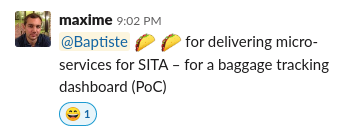
\includegraphics[scale=0.8]{tacos-usage}
            \caption{Utilisation d'un taco}\label{fig:taco}
        \end{figure}

        \subsection{Soft skills training}
        Tous les mercredis Siclo a choisi de prendre une heure trente sur la pause déjeuner pour entrainer tous les membres de 
        l'équipe aux \og soft skills\fg, dans le cadre de Siclo celà désigne
        surtout \emph{les compétences de communication}.
        L'objectif de ces séances étant principalement d'améliorer la
        communication au sein de l'équipe dans un contexte
        multiculturel\footnote{France/Vietnam}, mais également de savoir
        communiquer avec un client.

        \subsection{Dîner mensuel}
        Pour assurer la cohésion de toute l'équipe, un diner est organisé tous les mois avec tous les membres de l'équipe.
        Ce moment est aussi l'occasion de pouvoir voir chacun dans un contexte différent que pour le travail, avec notamment la possibilité
        d'échanger avec les membres vietnamiens de l'équipe, et ainsi mêler culture vetnamienne et française.
        Il est également courant d'y voir d'ancien membres de Siclo, c'est donc une occasion d'élargir son réseau dans une ambiance détendue
\end{document}
